\documentclass[10pt]{article}

\usepackage[margin=0.75in]{geometry}
\usepackage{amsmath, amssymb}
\usepackage{graphicx}
\usepackage[T1]{fontenc}
\usepackage{inconsolata}
\usepackage{titlesec}
\usepackage{fancyhdr}
\usepackage{microtype}
\usepackage{tikz}
\usetikzlibrary{arrows.meta}

\graphicspath{{../}}

\setlength{\parindent}{0pt}
\setlength{\parskip}{4pt}
\setlength{\tabcolsep}{4pt}
\renewcommand{\baselinestretch}{1.05}

\titleformat{\section}{\ttfamily\normalsize\bfseries\MakeUppercase}{\thesection}{0.6em}{}
\titlespacing*{\section}{0pt}{8pt}{2pt}
\titleformat{\subsection}{\ttfamily\small\MakeUppercase}{\thesubsection}{0.6em}{}
\titlespacing*{\subsection}{0pt}{6pt}{2pt}

\pagestyle{fancy}
\fancyhf{}
\renewcommand{\headrulewidth}{0pt}
\renewcommand{\footrulewidth}{0.5pt}
\fancyfoot[L]{\ttfamily\footnotesize BOND-ZONE-LOGIC}
\fancyfoot[C]{\ttfamily\footnotesize REV \today}
\fancyfoot[R]{\ttfamily\footnotesize \thepage}

\begin{document}

\noindent
\includegraphics[height=0.7cm]{logo}\hfill
{\ttfamily\normalsize\bfseries\MakeUppercase{Bond Zone Reinforcement Placement}}\quad
{\ttfamily\footnotesize\today}
\vspace{4pt}\hrule\vspace{6pt}

\section{Minimum Zone}

{\ttfamily\footnotesize
\begin{tabular}{@{}p{1.65in}p{5.05in}@{}}
Bars & \#5 minimum, \#11 maximum \\
Faces & provide the same rows each face of wall \\
Rows & 3 rows minimum each face \\
Cover & 1 in clear cover \\
Row spacing & 6 in on center after first row \\
\end{tabular}
}

\section{Row Layout}

{\ttfamily\footnotesize
\begin{tabular}{@{}p{1.55in}p{5.15in}@{}}
Straight edge & 3 rows each face: 1 in clear to bar edge, then 6 in o.c. \\
Overlap corner & 4 bars in the overlap box, 1 in clear from box/wall edges \\
Corner continuation & after the overlap box, offset row pairs at 6 in on center along each leg \\
\end{tabular}
}

\section{Placement Math}

\begin{equation}
e_b=c_{\text{clr}}+\frac{d_b}{2}
\end{equation}

{\ttfamily\footnotesize
\begin{tabular}{@{}ll@{}}
$e_b$ & bar centerline offset from concrete edge [in] \\
$c_{\text{clr}}$ & clear cover from concrete edge to nearest bar edge, use 1 in \\
$d_b$ & selected bar diameter [in] \\
\end{tabular}
}

\begin{equation}
r_k=e_b+(k-1)s_r, \qquad k=1,2,3
\end{equation}

{\ttfamily\footnotesize
\begin{tabular}{@{}ll@{}}
$r_k$ & straight-edge row $k$ centerline distance from wall edge [in] \\
$k$ & row index counted from wall edge \\
$s_r$ & row spacing, use 6 in on center \\
\end{tabular}
}

\begin{equation}
(x,y)\in\{(e_b,e_b),\ (b_x-e_b,e_b),\ (e_b,b_y-e_b),\ (b_x-e_b,b_y-e_b)\}
\end{equation}

{\ttfamily\footnotesize
\begin{tabular}{@{}ll@{}}
$x$ & local bar centerline coordinate along overlap-box width [in] \\
$y$ & local bar centerline coordinate along overlap-box depth [in] \\
$b_x$ & overlap-box width measured along the first wall leg [in] \\
$b_y$ & overlap-box depth measured along the second wall leg [in] \\
\end{tabular}
}

\begin{equation}
q_p=(b-e_b)+ps_r, \qquad p=1,2
\end{equation}

{\ttfamily\footnotesize
\begin{tabular}{@{}ll@{}}
$q_p$ & continuation-row centerline distance from overlap-box origin [in] \\
$b$ & overlap-box dimension along the continuing wall leg [in] \\
$p$ & continuation-row index outside overlap box \\
\end{tabular}
}

\medskip{\ttfamily\footnotesize\bfseries \#5 CENTER OFFSET}

{\ttfamily\footnotesize
\begin{tabular}{@{}ll@{}}
$d_b$ & 0.625 in \\
$e_b$ & 1.3125 in \\
\end{tabular}
}

\section{Rule}

{\ttfamily\footnotesize
\begin{tabular}{@{}p{0.35in}p{6.35in}@{}}
1 & Put bond-zone rows at wall ends, wall corners, and opening jamb edges. \\
2 & At a straight edge, place 3 rows minimum on each wall face. \\
3 & At an overlapping corner, place 4 bars in the corner overlap box. \\
4 & Keep corner-box bars 1 in clear to the bar edge, not to the bar centerline. \\
5 & From the corner box, continue row pairs at 6 in on center along each leg. \\
6 & Increase bar size only as needed, from \#5 up to \#11 maximum. \\
\end{tabular}
}

\section{Examples}

Straight-end groups have 6 bars minimum. Overlap-corner groups share the first row in a 4-bar box.

\medskip{\ttfamily\footnotesize\bfseries U WALL: 12 FT BY 12 FT}

{\ttfamily\footnotesize
\begin{tabular}{@{}p{2.25in}p{3.05in}r@{}}
Zone & Layout & Min bars \\
Left leg free end & 3 rows each face & 6 \\
Left/back overlap corner & 4-bar box + 2 row pairs each leg & 12 \\
Right/back overlap corner & 4-bar box + 2 row pairs each leg & 12 \\
Right leg free end & 3 rows each face & 6 \\
Total & 2 free ends + 2 overlap corners & 36 \\
\end{tabular}
}

\medskip{\ttfamily\footnotesize\bfseries L WALL: 16 FT BY 8 FT}

{\ttfamily\footnotesize
\begin{tabular}{@{}p{2.25in}p{3.05in}r@{}}
Zone & Layout & Min bars \\
Long leg free end & 3 rows each face & 6 \\
Overlap corner & 4-bar box + 2 row pairs each leg & 12 \\
Short leg free end & 3 rows each face & 6 \\
Total & 2 free ends + 1 overlap corner & 24 \\
\end{tabular}
}

\medskip{\ttfamily\footnotesize\bfseries T WALL: 15 FT WITH 8 FT MIDPOINT STEM}

{\ttfamily\footnotesize
\begin{tabular}{@{}p{2.25in}p{3.05in}r@{}}
Zone & Layout & Min bars \\
Left end of 15 ft wall & 3 rows each face & 6 \\
Right end of 15 ft wall & 3 rows each face & 6 \\
Stem free end & 3 rows each face & 6 \\
Midpoint overlap box & 4-bar box + 2 row pairs each branch & 16 \\
Total & 3 free ends + 1 three-branch overlap & 34 \\
\end{tabular}
}

\section{Cross Sections}

{\ttfamily\footnotesize
\begin{tabular}{@{}p{1.35in}p{5.35in}@{}}
Dot & one \#5 minimum bar position \\
Gray wall & schematic wall thickness; only cover and row spacing are being checked \\
Figure offset & dot centers drawn at 1.3125 in from concrete edge for \#5 bars \\
\end{tabular}
}

\medskip{\ttfamily\footnotesize\bfseries U WALL: 12 FT BY 12 FT}

\begin{center}
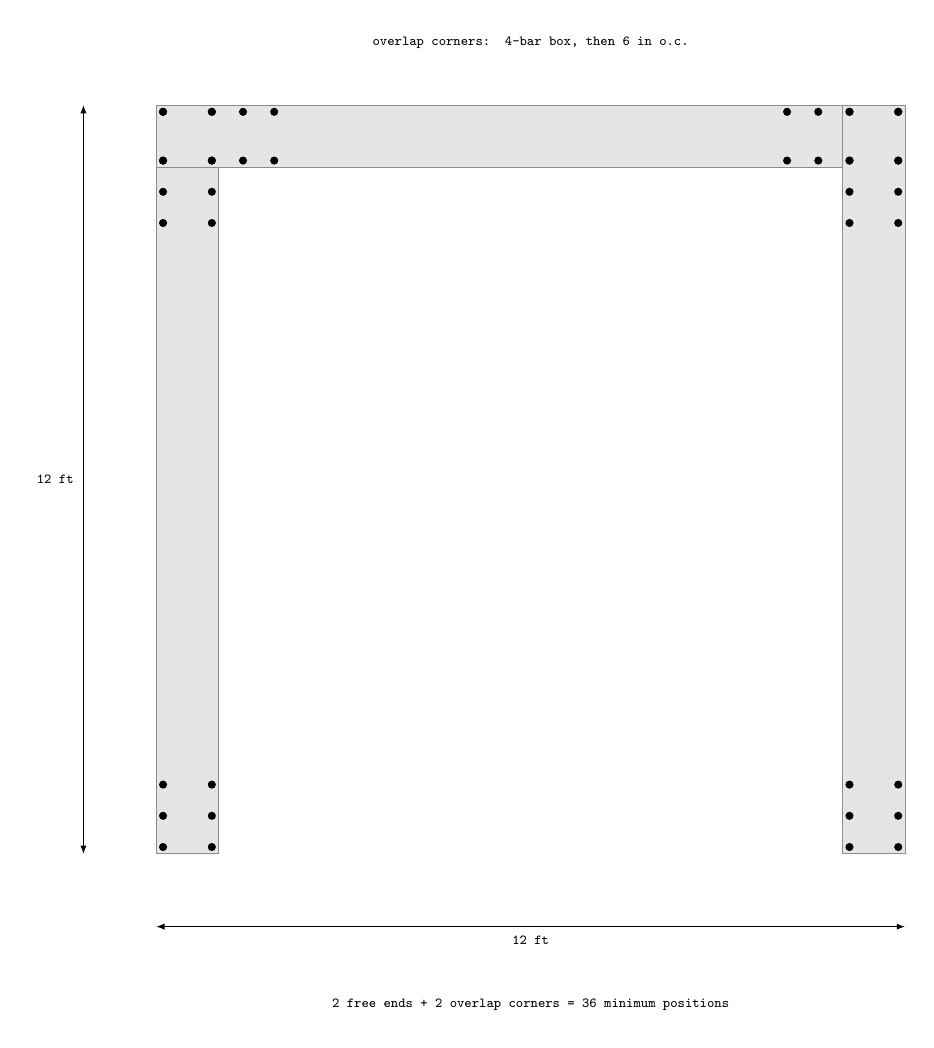
\begin{tikzpicture}[
  x=0.026in,
  y=0.026in,
  wall/.style={fill=black!10,draw=black!45,line width=0.35pt},
  bar/.style={fill=black,draw=black},
  dim/.style={{Latex[length=3pt]}-{Latex[length=3pt]},thin},
  lab/.style={font=\ttfamily\tiny}
]
\path[wall] (0,0) rectangle (12,144);
\path[wall] (0,132) rectangle (144,144);
\path[wall] (132,0) rectangle (144,144);
\foreach \y in {1.3125,7.3125,13.3125,121.3125,127.3125,133.3125,142.6875} {
  \fill[bar] (1.3125,\y) circle[radius=1.25pt];
  \fill[bar] (10.6875,\y) circle[radius=1.25pt];
  \fill[bar] (133.3125,\y) circle[radius=1.25pt];
  \fill[bar] (142.6875,\y) circle[radius=1.25pt];
}
\foreach \x in {1.3125,10.6875,16.6875,22.6875,121.3125,127.3125,133.3125,142.6875} {
  \fill[bar] (\x,133.3125) circle[radius=1.25pt];
  \fill[bar] (\x,142.6875) circle[radius=1.25pt];
}
\draw[dim] (0,-14) -- (144,-14) node[midway,below,lab]{12 ft};
\draw[dim] (-14,0) -- (-14,144) node[midway,left,lab]{12 ft};
\node[lab,below] at (72,-26) {2 free ends + 2 overlap corners = 36 minimum positions};
\node[lab,above] at (72,153) {overlap corners: 4-bar box, then 6 in o.c.};
\end{tikzpicture}
\end{center}

\medskip{\ttfamily\footnotesize\bfseries L WALL: 16 FT BY 8 FT}

\begin{center}
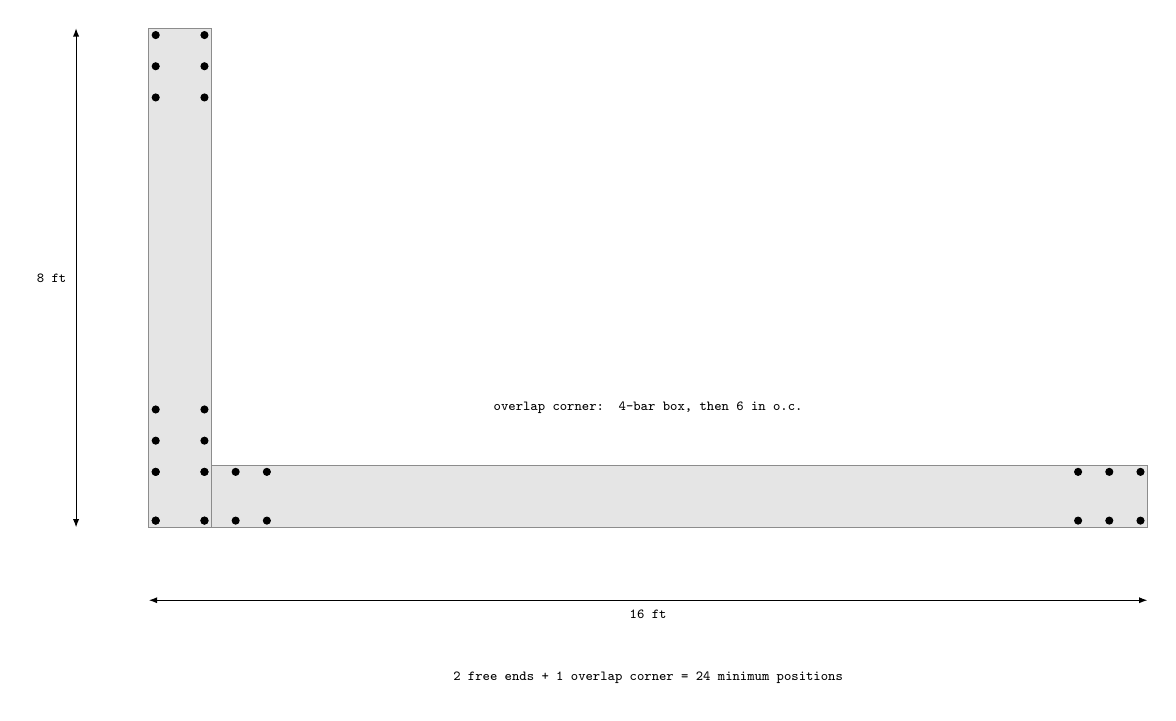
\begin{tikzpicture}[
  x=0.026in,
  y=0.026in,
  wall/.style={fill=black!10,draw=black!45,line width=0.35pt},
  bar/.style={fill=black,draw=black},
  dim/.style={{Latex[length=3pt]}-{Latex[length=3pt]},thin},
  lab/.style={font=\ttfamily\tiny}
]
\path[wall] (0,0) rectangle (192,12);
\path[wall] (0,0) rectangle (12,96);
\foreach \x in {1.3125,10.6875,16.6875,22.6875,178.6875,184.6875,190.6875} {
  \fill[bar] (\x,1.3125) circle[radius=1.25pt];
  \fill[bar] (\x,10.6875) circle[radius=1.25pt];
}
\foreach \y in {1.3125,10.6875,16.6875,22.6875,82.6875,88.6875,94.6875} {
  \fill[bar] (1.3125,\y) circle[radius=1.25pt];
  \fill[bar] (10.6875,\y) circle[radius=1.25pt];
}
\draw[dim] (0,-14) -- (192,-14) node[midway,below,lab]{16 ft};
\draw[dim] (-14,0) -- (-14,96) node[midway,left,lab]{8 ft};
\node[lab,below] at (96,-26) {2 free ends + 1 overlap corner = 24 minimum positions};
\node[lab,above] at (96,20) {overlap corner: 4-bar box, then 6 in o.c.};
\end{tikzpicture}
\end{center}

\medskip{\ttfamily\footnotesize\bfseries T WALL: 15 FT WITH 8 FT MIDPOINT STEM}

\begin{center}
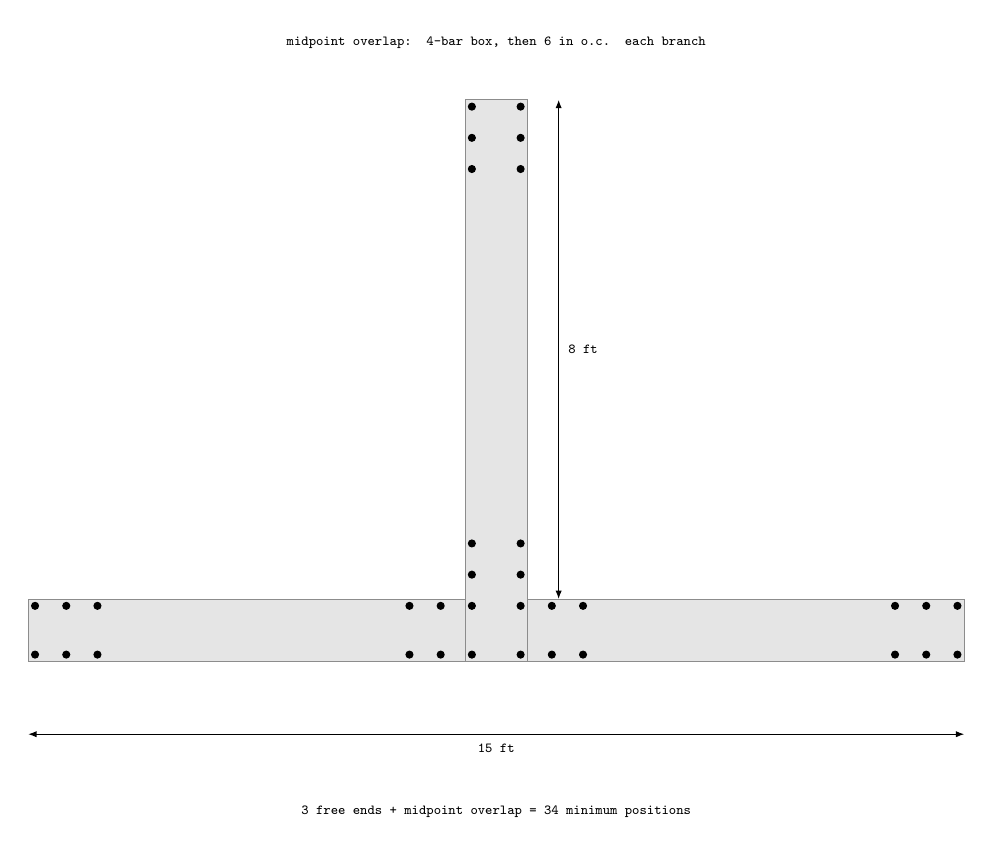
\begin{tikzpicture}[
  x=0.026in,
  y=0.026in,
  wall/.style={fill=black!10,draw=black!45,line width=0.35pt},
  bar/.style={fill=black,draw=black},
  dim/.style={{Latex[length=3pt]}-{Latex[length=3pt]},thin},
  lab/.style={font=\ttfamily\tiny}
]
\path[wall] (0,0) rectangle (180,12);
\path[wall] (84,0) rectangle (96,108);
\foreach \x in {1.3125,7.3125,13.3125,73.3125,79.3125,85.3125,94.6875,100.6875,106.6875,166.6875,172.6875,178.6875} {
  \fill[bar] (\x,1.3125) circle[radius=1.25pt];
  \fill[bar] (\x,10.6875) circle[radius=1.25pt];
}
\foreach \y in {16.6875,22.6875,94.6875,100.6875,106.6875} {
  \fill[bar] (85.3125,\y) circle[radius=1.25pt];
  \fill[bar] (94.6875,\y) circle[radius=1.25pt];
}
\draw[dim] (0,-14) -- (180,-14) node[midway,below,lab]{15 ft};
\draw[dim] (102,12) -- (102,108) node[midway,right,lab]{8 ft};
\node[lab,below] at (90,-26) {3 free ends + midpoint overlap = 34 minimum positions};
\node[lab,above] at (90,116) {midpoint overlap: 4-bar box, then 6 in o.c. each branch};
\end{tikzpicture}
\end{center}

\end{document}
